\documentclass[journal,12pt,twocolumn]{IEEEtran}
\usepackage{multicol}
\usepackage{blindtext}
\usepackage[shortlabels]{enumitem}
\usepackage{graphicx}
\usepackage{setspace}
\usepackage{gensymb}
\singlespacing
\usepackage[cmex10]{amsmath}
\usepackage{amssymb}
\usepackage{xurl}
\usepackage{tabularx}
\usepackage{amsthm}
\usepackage{comment}
\usepackage{mathrsfs}
\usepackage{txfonts}
\usepackage{stfloats}
\usepackage{bm}
\usepackage{cite}
\usepackage{cases}
\usepackage{subfig}
\usepackage{arydshln}
\usepackage{longtable}
\usepackage{multirow}

\usepackage{enumitem}
\usepackage{mathtools}
\usepackage{steinmetz}
\usepackage{tikz}
\usepackage{circuitikz}
\usepackage{verbatim}
\usepackage{tfrupee}
\usepackage[breaklinks=true]{hyperref}
\usepackage{graphicx}
\usepackage{tkz-euclide}
\usetikzlibrary{automata, positioning}
\usetikzlibrary{calc,math}
\usepackage{listings}
    \usepackage{color}                                            %%
    \usepackage{array}                                            %%
    \usepackage{longtable}                                        %%
    \usepackage{calc}                                             %%
    \usepackage{multirow}                                         %%
    \usepackage{hhline}                                           %%
    \usepackage{ifthen}                                           %%
    \usepackage{lscape}     
\usepackage{multicol}
\usepackage{chngcntr}
\usepackage{blkarray}

\DeclareMathOperator*{\Res}{Res}

\renewcommand\thesection{\arabic{section}}
\renewcommand\thesubsection{\thesection.\arabic{subsection}}
\renewcommand\thesubsubsection{\thesubsection.\arabic{subsubsection}}

\renewcommand\thesectiondis{\arabic{section}}
\renewcommand\thesubsectiondis{\thesectiondis.\arabic{subsection}}
\renewcommand\thesubsubsectiondis{\thesubsectiondis.\arabic{subsubsection}}


\hyphenation{op-tical net-works semi-conduc-tor}
\def\inputGnumericTable{}                                 %%

\lstset{
%language=C,
frame=single, 
breaklines=true,
columns=fullflexible
}



\begin{document}


\newtheorem{theorem}{Theorem}[section]
\newtheorem{problem}{Problem}
\newtheorem{proposition}{Proposition}[section]
\newtheorem{lemma}{Lemma}[section]
\newtheorem{corollary}[theorem]{Corollary}
\newtheorem{example}{Example}[section]
\newtheorem{definition}[problem]{Definition}

\newcommand{\BEQA}{\begin{eqnarray}}
\newcommand{\EEQA}{\end{eqnarray}}
\newcommand{\define}{\stackrel{\triangle}{=}}
\bibliographystyle{IEEEtran}
\raggedbottom
\setlength{\parindent}{0pt}
\providecommand{\mbf}{\mathbf}
\providecommand{\pr}[1]{\ensuremath{\Pr\left(#1\right)}}
\providecommand{\qfunc}[1]{\ensuremath{Q\left(#1\right)}}
\providecommand{\sbrak}[1]{\ensuremath{{}\left[#1\right]}}
\providecommand{\lsbrak}[1]{\ensuremath{{}\left[#1\right.}}
\providecommand{\rsbrak}[1]{\ensuremath{{}\left.#1\right]}}
\providecommand{\brak}[1]{\ensuremath{\left(#1\right)}}
\providecommand{\lbrak}[1]{\ensuremath{\left(#1\right.}}
\providecommand{\rbrak}[1]{\ensuremath{\left.#1\right)}}
\providecommand{\cbrak}[1]{\ensuremath{\left\{#1\right\}}}
\providecommand{\lcbrak}[1]{\ensuremath{\left\{#1\right.}}
\providecommand{\rcbrak}[1]{\ensuremath{\left.#1\right\}}}
\theoremstyle{remark}
\newtheorem{rem}{Remark}
\newcommand{\sgn}{\mathop{\mathrm{sgn}}}
\providecommand{\abs}[1]{\vert#1\vert}
\providecommand{\res}[1]{\Res\displaylimits_{#1}} 
\providecommand{\norm}[1]{\lVert#1\rVert}
%\providecommand{\norm}[1]{\lVert#1\rVert}
\providecommand{\mtx}[1]{\mathbf{#1}}
\providecommand{\mean}[1]{E[ #1 ]}
\providecommand{\fourier}{\overset{\mathcal{F}}{ \rightleftharpoons}}
%\providecommand{\hilbert}{\overset{\mathcal{H}}{ \rightleftharpoons}}
\providecommand{\system}{\overset{\mathcal{H}}{ \longleftrightarrow}}
	%\newcommand{\solution}[2]{\textbf{Solution:}{#1}}
\newcommand{\solution}{\noindent \textbf{Solution: }}
\newcommand{\cosec}{\,\text{cosec}\,}
\providecommand{\dec}[2]{\ensuremath{\overset{#1}{\underset{#2}{\gtrless}}}}
\newcommand{\myvec}[1]{\ensuremath{\begin{pmatrix}#1\end{pmatrix}}}
\newcommand{\mydet}[1]{\ensuremath{\begin{vmatrix}#1\end{vmatrix}}}
\newcommand*{\permcomb}[4][0mu]{{{}^{#3}\mkern#1#2_{#4}}}
\newcommand*{\perm}[1][-3mu]{\permcomb[#1]{P}}
\newcommand*{\comb}[1][-1mu]{\permcomb[#1]{C}}
\numberwithin{equation}{subsection}
\makeatletter
\@addtoreset{figure}{problem}
\makeatother
\let\StandardTheFigure\thefigure
\let\vec\mathbf
\renewcommand{\thefigure}{\theproblem}
\def\putbox#1#2#3{\makebox[0in][l]{\makebox[#1][l]{}\raisebox{\baselineskip}[0in][0in]{\raisebox{#2}[0in][0in]{#3}}}}
     \def\rightbox#1{\makebox[0in][r]{#1}}
     \def\centbox#1{\makebox[0in]{#1}}
     \def\topbox#1{\raisebox{-\baselineskip}[0in][0in]{#1}}
     \def\midbox#1{\raisebox{-0.5\baselineskip}[0in][0in]{#1}}
\vspace{3cm}
\title{\textbf{LINEAR SYSTEMS AND SIGNAL PROCESSING \\ QUIZ 2}}
\author{GANJI VARSHITHA - AI20BTECH11009}
\maketitle
\newpage
\bigskip
\renewcommand{\thefigure}{\arabic{figure}}
\renewcommand{\thetable}{\arabic{table}}
Download latex codes from 
%
\begin{lstlisting}
https://github.com/VARSHITHAGANJI/EE3900_GATE_ASSIGNMENTS/blob/main/QUIZ2/QUIZ2.tex
\end{lstlisting}
Download all python codes from
\begin{lstlisting}
https://github.com/VARSHITHAGANJI/EE3900_GATE_ASSIGNMENTS/blob/main/QUIZ2/quiz2code.py
\end{lstlisting}
\section*{QUESTION}
\textbf{Problem 3.24(b)}
Sketch each of the following sequences and determine their $z$- transforms, including the region of convergence
\begin{enumerate}[(a)]
\item $\sum_{k=-\infty}^{\infty} \delta\sbrak{n-k}$
\item $\frac{1}{2}\sbrak{e^{j\pi n} + cos\brak{\frac{\pi}{2} n} + \sin\brak{\frac{\pi}{2}+2 \pi n}}u\sbrak{n}$

\end{enumerate}
\section*{SOLUTION}
(b)\\
Let 
\begin{align}
\label{eq:1}
a\sbrak{n}={}& \frac{1}{2}\sbrak{e^{j\pi n} + \cos\brak{\frac{\pi}{2} n} + \sin\brak{\frac{\pi}{2}+2 \pi n}}u\sbrak{n}
\end{align}

We have 
\begin{align}
\label{eq:2}
e^{j \pi n} ={}& \brak{-1}^n \forall n\\
\label{eq:3}
\sin\brak{\frac{\pi}{2}+2 \pi n} = {}& 1 \forall n\\
\label{eq:4}
u\sbrak{n}={}& \left\{
  \begin{array}{lr} 
      1, & n\geq 0 \\
      0, & \text{ otherwise }
      \end{array}
\right.
\end{align}
\begin{align}
\label{eq:5}
\cos\brak{\frac{\pi}{2} n} = {}& \left\{
  \begin{array}{lr} 
      1, & n = 4k,\; k\geq 0 \\
      -1, & n = 4k+2,\; k \geq 0 \\
      0, & \text{ otherwise }
      \end{array}
\right.
\end{align}

Substituting \eqref{eq:2}, \eqref{eq:3},\eqref{eq:4} and \eqref{eq:5} in \eqref{eq:1}, we get 
Let 
\begin{align}
\label{eq:6}
a\sbrak{n} ={}& \frac{1}{2}\sbrak{\brak{-1}^{n} + \cos\brak{\frac{\pi}{2} n} + 1}u\sbrak{n}\\
\label{eq:7}
={}& \left\{
  \begin{array}{lr} 
      \frac{3}{2}, & n = 4k,\; k\geq 0 \\
      \frac{1}{2}, & n = 4k+2,\; k \geq 0 \\
      0, & \text{ otherwise }
      \end{array}
\right.
\end{align}
Let the $z$-transform of $a\sbrak{n}$ be $A\brak{z}$.\\
By definition of $z$-transform, we have
\begin{align}
\label{eq:8}
A\brak{z}={}& \sum_{n=-\infty}^\infty a\sbrak{n}z^{-n}
\end{align}
As $u\sbrak{n} = 0\: \forall n< 0$
\begin{align}
\label{eq:9}
A\brak{z}={}& \sum_{n=0}^\infty a\sbrak{n}z^{-n}
\end{align}
Let the sequence be $a_{1}\sbrak{n}$ for n = 4k and $a_{2}\sbrak{n}$ for n= 4k+2. \\
Let their corresponding $z$-transforms be $A_{1}\brak{z}$ and $A_{2}\brak{z}$ respectively.\\
Take $k=\frac{n}{4}$
\begin{align}
\label{eq:10}
A_{1}\brak{z} = {}& \sum_{k=0}^\infty a_{1}\sbrak{n}z^{-4k}\\
\label{eq:11}
={}& \sum_{k=0}^\infty \frac{3}{2}z^{-4k}\\
\label{eq:12}
={}& \frac{\frac{3}{2}}{1-z^{-4}}
\end{align}
ROC is $|z|>1$.\\
Take $k=\frac{n-2}{4}$
\begin{align}
\label{eq:13}
A_{2}\brak{z} = {}& \sum_{k=0}^\infty a_{2}\sbrak{n}z^{-4k-2}\\
\label{eq:14}
={}& \sum_{k=0}^\infty \frac{1}{2}z^{-2}z^{-4k}\\
\label{eq:15}
={}& \frac{\frac{1}{2}z^{-2}}{1-z^{-4}}
\end{align}
ROC is $|z|>1$.\\
Since $A\brak{z}= A_{1}\brak{z} + A_{2}\brak{z}$,
\begin{align}
A\brak{z} ={}& \frac{\frac{3}{2}+\frac{1}{2}z^{-2}}{1-z^{-4}}
\end{align}
ROC is $|z|>1$.
\begin{figure}[h]
\centering
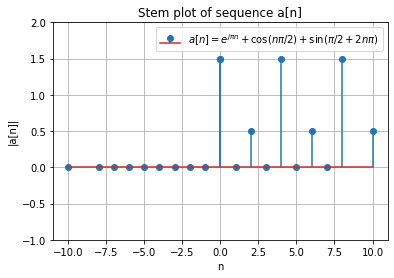
\includegraphics[width = \columnwidth]{q2_quiz2}
\end{figure}





\end{document}
